\documentclass[main.tex,fontsize=8pt,paper=a4,paper=portrait,DIV=calc,]{scrartcl}
% Document
\usepackage[T1]{fontenc}
\usepackage[dvipsnames]{xcolor}
\usepackage[nswissgerman,english]{babel}
\renewcommand{\familydefault}{\sfdefault}

% Format
\usepackage[top=5mm,bottom=1mm,left=5mm,right=5mm]{geometry}
%\setlength{\headheight}{\baselineskip}
%\setlength{\headsep}{0mm}

%\usepackage{scrlayer-scrpage}
%\clearpairofpagestyles
%\chead{{\bfseries\TITLE, \AUTHOR, \pagename~\thepage}}

%\addtokomafont{pagehead}{\upshape}

\usepackage{multicol}
\setlength{\columnsep}{2mm}
\setlength{\columnseprule}{0.1pt}

% Math
\usepackage{amsmath}
\usepackage{amssymb}
\usepackage{amsfonts}

% Code
\usepackage{fancyvrb, etoolbox, listings, xcolor}
%\usemintedstyle{bw}

%\newminted[shell]{bash}{
%fontsize=\footnotesize,
%fontfamily=tt,
%breaklines=true,
%frame=single,
%framerule=0.1pt,
%framesep=2mm,
%tabsize=2
%}
%\newminted{css}{
%breaklines=true,
%tabsize=4,
%autogobble=true,
%escapeinside=||,
%stripall=true,
%stripnl=true,
%}

    \definecolor{lightgray}{rgb}{0.95, 0.95, 0.95}
    \definecolor{darkgray}{rgb}{0.4, 0.4, 0.4}
    \definecolor{purple}{rgb}{0.65, 0.12, 0.82}
    \definecolor{ocherCode}{rgb}{1, 0.5, 0} % #FF7F00 -> rgb(239, 169, 0)
    \definecolor{blueCode}{rgb}{0, 0, 0.93} % #0000EE -> rgb(0, 0, 238)
    \definecolor{greenCode}{rgb}{0, 0.6, 0} % #009900 -> rgb(0, 153, 0)
    \definecolor{teal}{rgb}{0.0, 0.5, 0.5}

\lstdefinestyle{code}{
    identifierstyle=\color{black},
    keywordstyle=\color{blue}\bfseries\small,
    ndkeywordstyle=\color{greenCode}\bfseries\small,
    stringstyle=\color{ocherCode}\ttfamily\small,
    commentstyle=\color{teal}\ttfamily\textit\small,
    basicstyle=\ttfamily\small,
    breakatwhitespace=false,         
    breaklines=true,                 
    captionpos=b,                    
    keepspaces=true,                 
    showspaces=false,                
    showstringspaces=false,
    showtabs=false,                  
    tabsize=2,
    belowskip=-5pt
}



% Images
\usepackage{graphicx}
\newcommand{\pic}{\includegraphics[scale=0.3]}
\graphicspath{{Screenshots/}{../Screenshots}}
\makeatletter
\def\pictext#1#2{%
    \@ifnextchar[{%
    \pictext@iiiii{#1}{#2}%
    }{%
      \pictext@iiiii{#1}{#2}[0.5,0.4,0.3]% Default is 5
    }%
}
\def\pictext@iiiii#1#2[#3,#4,#5]{\begin{minipage}{#3\textwidth}\includegraphics[scale=#4]{#1}\end{minipage}\begin{minipage}{#5\textwidth}#2\end{minipage}}
\def\minipg#1#2{%
    \@ifnextchar[{%
    \minipg@iiii{#1}{#2}%
    }{%
      \minipg@iiii{#1}{#2}[0.3,0.6]% Default is 5
    }%
}
\def\minipg@iiii#1#2[#3,#4]{\vspace{0.8mm}\begin{minipage}{#3\textwidth}#1\end{minipage}\begin{minipage}{#4\textwidth}#2\end{minipage}{\vspace{0.8mm}}}
\makeatother

%\newenvironment{minty}[2]% environment name
%{% begin code
%  \begin{minipage}{#1}
%  \begin{minted}{#2}
%}%
%{% end code
%  \end{minted}
%  \end{minipage}
%  \end{minty}\ignorespacesafterend
%} 

% Smaller Lists
\usepackage{enumitem}
\setlist[itemize,enumerate]{leftmargin=3mm, labelindent=0mm, labelwidth=1mm, labelsep=1mm, nosep}
\setlist[description]{leftmargin=0mm, nosep}
\setlength{\parindent}{0cm}

% Smaller Titles
\usepackage[explicit]{titlesec}

%% Color Boxes
\newcommand{\sectioncolor}[1]{\colorbox{black!60}{\parbox{0.989\linewidth}{\color{white}#1}}}
\newcommand{\subsectioncolor}[1]{\colorbox{black!50}{\parbox{0.989\linewidth}{\color{white}#1}}}
\newcommand{\subsubsectioncolor}[1]{\colorbox{black!40}{\parbox{0.989\linewidth}{\color{white}#1}}}
\newcommand{\paragraphcolor}[1]{\colorbox{black!30}{\parbox{0.989\linewidth}{\color{white}#1}}}
\newcommand{\subparagraphcolor}[1]{\colorbox{black!20}{\parbox{0.989\linewidth}{\color{white}#1}}}

%% Title Format
\titleformat{\section}{\vspace{0.5mm}\bfseries}{}{0mm}{\sectioncolor{\thesection~#1}}[{\vspace{0.5mm}}]
\titleformat{\subsection}{\vspace{0.5mm}\bfseries}{}{0mm}{\subsectioncolor{\thesubsection~#1}}[{\vspace{0.5mm}}]
\titleformat{\subsubsection}{\vspace{0.5mm}\bfseries}{}{0mm}{\subsubsectioncolor{\thesubsubsection~#1}}[{\vspace{0.5mm}}]
\titleformat{\paragraph}{\vspace{0.5mm}\bfseries}{}{0mm}{\paragraphcolor{\theparagraph~#1}}[{\vspace{0.5mm}}]
\titleformat{\subparagraph}{\vspace{0.5mm}\bfseries}{}{0mm}{\subparagraphcolor{\thesubparagraph~#1}}[{\vspace{0.5mm}}]

%% Title Spacing
\titlespacing{\section}{0mm}{0mm}{0mm}
\titlespacing{\subsection}{0mm}{0mm}{0mm}
\titlespacing{\subsubsection}{0mm}{0mm}{0mm}
\titlespacing{\paragraph}{0mm}{0mm}{0mm}
\titlespacing{\subparagraph}{0mm}{0mm}{0mm}

%% format cells
\usepackage[document]{ragged2e}
\usepackage{array, makecell}
\renewcommand{\arraystretch}{2}
\newcommand{\mc}{\makecell[{{m{1\linewidth}}}]}


\usepackage{listings-rust}

\lstset{
    language=Rust,
    style=colouredRust,
}
%%%%%

\begin{document}
\begin{table}[h!]
\section{Cargo}
\begin{tabular}{|m{0.2\linewidth}|m{0.755\linewidth}|}
\hline
Default Commands &
\vspace{2mm}
\begin{itemize}
  \item \textcolor{teal}{Cargo new} creates a new rust project with git integration
  \item \textcolor{teal}{Cargo build} build a project if the toml file has been provided
  \item \textcolor{teal}{Cargo build --release} builds the release version without debugging environment
  \item \textcolor{teal}{Cargo run} runs the project
  \item \textcolor{teal}{Cargo check} this only checks the code if it would compile! But it doesn't actually compile! Super helpful!
  \vspace{-3mm}
\end{itemize}\\
\hline
Toml & 
\begin{lstlisting}
[package]
name = "hello_cargo"
version = "0.1.0"
edition = "2021"

[dependencies]
\end{lstlisting}
\\
\hline
\end{tabular}
\section{Basic Terms and Information}
\begin{tabular}{|m{0.2\linewidth}|m{0.755\linewidth}|}
\hline
Comments & 
\textcolor{orange}{Comments are made with // just like C++ or C}\\
\hline
Main & 
\textcolor{orange}{Just like c++, the first function is always main!}\newline
\textcolor{teal}{However, unlike c++ the function definition order doesn't matter, there is no need for hpp files or similar!}\newline
\textcolor{purple}{The function main always needs to return either 0 -> () or -> Result<(), E> (this type is explained further below in error handling).}\newline
\textcolor{purple}{the underlying convention of Result<(), E> is either return 0 aka () if ok, or return some other integer in case of error\newline
You can however also return other types, that implement the "std::process::Termination" trait (also explained later)}\\
\hline
Naming convention & 
\vspace{2mm}
\begin{itemize}
  \item \textcolor{teal}{Functions: some\_function\_name()}
  \item \textcolor{teal}{}
  \item \textcolor{teal}{}
  \item \textcolor{teal}{}
  \vspace{-3mm}
\end{itemize}\\
\hline
\textbf{Macros} & 
\textcolor{orange}{You use a macro with the "!" keyword after a function}\newline
\begin{lstlisting}
fn main() {
    println!("Henlo birb!");
}
\end{lstlisting}\\
\hline
Variable definition & 
\textcolor{orange}{Rust has a peculiar syntax for writing variables, it is very much different to all other languages}\newline
\begin{lstlisting}
let num = 5; 
// this produces an immutable variable num, yes IMMUTABLE!!

let mut num2 = 5;
// num2 is MUTABLE because of the mut keyword!!

let mut num3: u32 = 5;
// this specifies a type of u32 int to the variable!
\end{lstlisting}\\
\hline
Strings & 
\textcolor{orange}{Strings in rust are strange, they are declared as follows:}\newline
\begin{lstlisting}
let mut grief = String::new();
// empty string

let mut grief = String::from("grief");
// mutable string with value "grief"
\end{lstlisting}
\, \newline
\textcolor{teal}{However, there are also trivial strings, they just do not have all the functions of the other strings.\newline
They do however in contrast work just like regular strings in c++.}\newline
\begin{lstlisting}
let mut str = "ping";
println!("{str}"); //prints ping
str += "pang";
println!("{str}"); //prints pingpang
\end{lstlisting}\\
\hline
\end{tabular}
\end{table}
\pagebreak
\begin{table}[ht!]
\begin{tabular}{|m{0.2\linewidth}|m{0.755\linewidth}|}
\hline
Input \& Output & 
\begin{lstlisting}
std::io::stdin()
         .read_line(&mut num2)
         .expect("Failed to read line");
// the &mut is needed to reference the num2 variable as a mutable reference
// This string has by default an added newline,
// to get rid of this we have to format it
let num2 = num2.trim();
// this will create a new num2 variable and ghost the last one!!!
// .trim() will remove all whitespaces at the front and at the back
// just like definition it is by default immutable
// expect will trigger if the input has failed

// interesting is also the printing of variables inside println!
println!("The number is {num2}")
println!("The number is {},num2")
// these are identical! 
// If you have multiple numbers you have to order them in the same way as the empty {} are.
\end{lstlisting}
\, \newline
\textcolor{orange}{Similar to C++ we need namespaces to use standard library functions}\newline
\textcolor{teal}{.read\_line() has a result of either "Ok", or "Err" which must be handled with the .expected() function! \newline
This apparently will (guess) throw an error}\\
\hline
\end{tabular}
\end{table}
\pagebreak
\begin{table}[ht!]
\begin{tabular}{|m{0.2\linewidth}|m{0.755\linewidth}|}
\hline
conditional on Input & 
\textcolor{orange}{Instead of just parsing a string,\newline
we can also use functions on fail or ok states!}\newline
\begin{lstlisting}
loop {
    let mut guess = String::new();
    std::io::stdin()
        .read_line(&mut guess)
        .expect("failed to read line")
    
    let guess: u32 = match guess.trim().parse() { // match the parsed string
        Ok(num) => num, // if the string is a u32 int, then create the var num with that value
        Err(_) => continue, // continue the loop if it is not a u32 int
    }

}
\end{lstlisting}\\
\hline
loops & 
\textcolor{orange}{The easiest but also silliest loop in rust is the simple keyword: \textbf{loop}, it creates an infinite loop!}\newline
\begin{lstlisting}
loop {
    println!("I will print ping pang until you close the program!");
}
\end{lstlisting}\\
\hline
comparisons & 
\textcolor{orange}{Rust allows for a strange comparison syntax:}\newline
\begin{lstlisting}
loop {
    match guess.cmp(&secret_number) {
        Ordering::Less => println!("Too small!"), // do if guess is smaller
        Ordering::Greater => println!("Too big!"), // do if guess is bigger
        Ordering::Equal => { // do if guess is same!
            println!("You win!");
            break; // break loop
        }
    }
}
// Theoretically this is the same as a bunch of if-statements,
// however, I have no idea how the performance compapres....
\end{lstlisting}\\
\hline
random numbers & 
\textcolor{orange}{Unlike C or C++ you do not need to provide a seed.\newline
Just like in python you can simply use the rand function:}\newline
\begin{lstlisting}
let secret_number = rand::Rng::treadh_rng().gen_range(1..=100);
// this creates a rnadom number with range 1 to and with 100.
\end{lstlisting}\\
\hline
Constants & 
\begin{lstlisting}
cont SOME_CONSTANT: u32 = 5;
\end{lstlisting}\\
\hline
Scopes and Shadowing & 
\textcolor{orange}{Just like c++, when we have scopes and we redefine a variable, then it will only overwrite said variable in that scope.}\newline 
\begin{lstlisting}
let x = 5;
{ // empty scope
    let x = 10;
    println!({&x});
    // prints 10
}
println!({$x});
// prints 5
\end{lstlisting}
\, \newline
\textcolor{teal}{Interesting to know, you can create another variable with a different type and the same name!\newline 
This will still just shadow the previous one, \textbf{HOWEVER}, }\textcolor{red}{Shadowing does \textbf{NOT work with mutable variables!}}\newline
\begin{lstlisting}
let x = 5;
let x = "ping";
// OK
let mut y = 5;
let mut y = "ping";
// ERROR! can't shadow mutable variable
\end{lstlisting}\\
\hline 
Integer Sizes& 
\vspace{2mm}
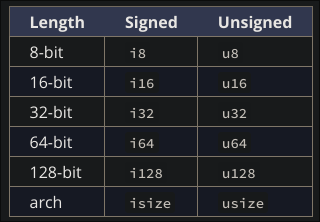
\includegraphics[scale=0.45]{2022-10-19-01:21:45.png}
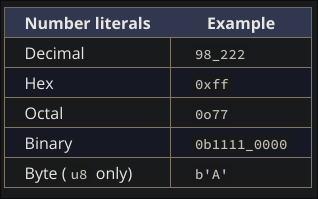
\includegraphics[scale=0.45]{2022-10-19-01:25:19.png}\newline
\textcolor{orange}{The default is i32 integer}
\\
\hline
\end{tabular}
\end{table}
\pagebreak
\begin{table}[ht!]
\begin{tabular}{|m{0.2\linewidth}|m{0.755\linewidth}|}
\hline
Float and double & 
\textcolor{orange}{In rust double is the default floating point type!}\newline
\begin{lstlisting}
let x = 5.5; // has type f64 -> double
let x: f32 = 5.5; // this is a float -> float is f32
\end{lstlisting}
\, \newline 
\textcolor{teal}{Note for calculations, just like in c++ if you do divisions,
make sure you use floats, unless you want truncated values:}\newline
\begin{lstlisting}
let x = 5 / 2;
// x = 2!
let x = 5.0 / 2.0;
// x = 2.5
\end{lstlisting}
\\
\hline
Chars & 
\begin{lstlisting}
fn main() {
    let c = 'z';
    let z: char = 'Z'; // with explicit type annotation
    let heart_eyed_cat = 'emoj';
    // latex might not show it, but you can insert emojis....
}
\end{lstlisting}\\
\hline
Tuples & 
\textcolor{orange}{Tuples are very easy in rust!}\newline
\begin{lstlisting}
    // creating a tuple
    let tup: (i32, f64, u8) = (500, 6.4, 1);

    //accessing a tuple
    let num = tup.1;
    // assigns the first value of tup -> num = 500
    // tup.2 -> 6.4, tup.3 -> 1

    let tup2 = (500, 6.4, 1);
    let (x, y, z) = tup2;
    // assign x = 500, y = 6.4, z = 1
\end{lstlisting}\\
\hline
Arrays & 
\begin{lstlisting}
// creating arrays
let arr = [1,2,3,4,5];
// implicit type and size
let arr2: [i32;5] = [1,2,3,4,5];
// explicit type and size
let arr3 = [3;5];
// creates an array of: [3,3,3,3,3] 5 times the value 3

// accessing arrays -> done just like c++
// arr[0] -> 1
// arr[1] -> 2
// should you go out of bounds, it will panick -> runtime error
\end{lstlisting}\\
\hline
Function Parameters &
\textcolor{orange}{Function parameters are always explicit!}\newline
\begin{lstlisting}
fn some_func(x: i32, y: char) {
    println!("value of {y} is {x}");
}
some_func(5,'h');
\end{lstlisting}\\
\hline
Scopes in rust & 
\begin{lstlisting}
let y = {
        let x = 3;
        x + 1 // no error this works because of the scope!
    }; // it's essentially a return statement!

println!("The value of y is: {y}");
// will print the value 4
\end{lstlisting}\\
\hline
\textbf{Return} & 
\textcolor{orange}{\textbf{In Rust functions can return values implicitly, and it is also used like this!}}\newline
\begin{lstlisting}
fn ret() -> i32 { // you must specify the return like this! i32 for int
    5
}
// this function simply returns 5 !!
fn ret2() -> (i32, String) {
    (5, "henlo birb!") // Rust allows you to return tuples as well!!
}
\end{lstlisting}
\, \newline
\textcolor{teal}{You can still use the return keyword in rust, it is just not needed -> choose a style...}\newline
\textcolor{red}{\textbf{More importantly: the return value MUST be written and it is after an arrow: \emph{->}}}\\
\hline
\end{tabular}
\end{table}
\pagebreak
\begin{table}[ht!]
\begin{tabular}{|m{0.2\linewidth}|m{0.755\linewidth}|}
\hline
Expressions vs Statements &
\textcolor{red}{\textbf{VERY IMPORTANT, rust makes a clear difference between an expression and a statement.}}\newline
\textcolor{orange}{A statement is something like a variable to return in a function, while an expression is something like a function call some\_func()}\newline
\textcolor{red}{\textbf{So, yes, when returning a value you do not put a semicolon at the end!}}\newline
\begin{lstlisting}
fn some_func() -> i32 {
    5 // NO SEMICOLON!!!!!
    5; // WRONG!!!!
}
\end{lstlisting}\\
\hline
If statements & 
\textcolor{orange}{In rust if statements do not need brackets around them, the compiler even tells you about unnecessary brackets!}\newline
\begin{lstlisting}
if x > 5 {
    println!("ping pang");
} else {
    println!("sadly no pang ping");
}
\end{lstlisting}
\, \newline
\textcolor{teal}{There is one more caviat, since rust does not do implicit type conversion if there is data loss, it also doesn't convert integers to booleans!}
\begin{lstlisting}
let x = 5;
if x {
 // doesn't work !!! error implicit cast not allowed!
}
if x != 0 {
 // works
}
\end{lstlisting}\\
\hline
Inline If & 
\textcolor{teal}{You can also write inline if statements to for example assign a value to a variable:}\newline
\begin{lstlisting}
let x = 5;
let y = if x > 6 {4} else {3};
// y now has the value of 3 as x is not greater than 6
\end{lstlisting}\\
\hline
Loops & 
\textcolor{orange}{Prepare for brainfuck, loops in rust are super weird, here an example with comparison to c++}\newline
\textcolor{teal}{Note that this can be done differently with a for loop in c++!}\newline
\begin{lstlisting}
fn main() {                                    void main() {        
    let mut counter = 0;                           int result = 0;
                                                   int counter = 0;
    let result = loop {                            while (true) {
        counter += 1;                                  if (counter == 10) { 
                                                          result = counter * 2;
        if counter == 10 {                             } 
            break counter * 2;                     counter += 1;
        // <<< result = counter * 2 !!!!          }
        }                                      std::cout << "The result is " << result << "\n";
    };                                         }
    println!("The result is {result}");       
}
\end{lstlisting}
\, \newline
\textcolor{orange}{Take a close look at the break counter * 2, this is essentially a return statement from a loop that will be assigned to the variable result.}\\
\hline
Loops with labels &
\textcolor{orange}{Another quirk with loops in rust is that you can assign labels to loops, this is needed to break out of a loop without assigning a value!}\newline
\begin{lstlisting}
let mut counter = 0;
'some_name: loop { // notice the ' at the start !!!!
    if counter == 2 {
        break 'some_name; // break the loop with label some_name
        // this means you can break loops nested loops!!!!
    }
    counter += 1;
}
\end{lstlisting}\\
\hline
While Loops &
\textcolor{teal}{While loops are the same as c++ without the brackets.}\newline
\begin{lstlisting}
let mut counter = 0;
while counter != 3 {
    counter += 1;
    println!({counter});
}
\end{lstlisting}\\
\hline
\end{tabular}
\end{table}
\pagebreak
\begin{table}[ht!]
\begin{tabular}{|m{0.2\linewidth}|m{0.755\linewidth}|}
\hline
For Loops &
\textcolor{teal}{For loops can be used like ranged based for loops in c++ and co.}\newline
\begin{lstlisting}
let x = [1,2,3,4,5];
for element in x {
    println!({element});
}
\end{lstlisting}
\, \newline
\textcolor{orange}{For loops like this for (int i = 0; i < x.size; i++), you write the following:}\newline
\begin{lstlisting}
for number in (1..x.size()).rev() { // x.size == 4
    // instead of x.size you can put any number there !
    println!("{number}!");
}
\end{lstlisting}\\
\hline
\textbf{\textcolor{red}{Ownership}} & 
\textcolor{orange}{This is the reason you use rust, it is the management of ownership that makes rust both safe and fast. It is a third approach to memory handling next to the known garbage collector system and the raw pointer approach from c and c++}\newline
\textcolor{teal}{The ownership system states, that each heap value must always have an owner, if this requirement is not fulfilled, then the value will be dropped.\newline
This can be compared to a pointer in c++ with the only difference being the fact that the value in c++ can have no pointer as well -> PROBABLE MEMORY LEAK!}\newline
\textcolor{red}{Here is a list of rules that you must follow when programming in rust:} \newline
\begin{enumerate}
\item \textcolor{teal}{\textbf{Each heap value must ALWAYS have an owner}}
\item \textcolor{teal}{\textbf{Each heap value can only have 1 owner at a time}}
\item \textcolor{teal}{\textbf{The owner can change!}}
\item \textcolor{teal}{\textbf{If a value loses it's owner without a replacement, the value will be dropped -> deleted from memory}}
\vspace{-3mm}
\end{enumerate}
\\
\hline
Heap allocated variables & 
\textcolor{orange}{In rust heap allocated variables are essentially just pointers, similar to how java handles them, however, unlike java, rust only allows 1 variable to reference the heap.\newline
As already stated above, only 1 owner may be present at any time.\newline
This result in the following scenario:}\newline
\begin{lstlisting}
    let s1 = String::from("hello"); // declare the heap allocated string s1
    let s2 = s1; // declare s2 with the values at the memory address s1 points to
                 // ownership is transfered to s2! therefore >>s1 IS OUT OF SCOPE<<
    println!("{}, world!", s1); // ERROR s1 is dropped, aka it is no longer defined!
\end{lstlisting}
\, \newline
\textcolor{red}{This behavior not only makes sense, it also enforces move semantics, as you can't make endless copies of pointers that are unnecessary! \newline
But it also makes sure that you don't make copies implicitly with new constructors!}\\
\hline
Copying Heap variables & 
\textcolor{orange}{Of course, you can still copy the data of heap allocated variables should you wish to have it this way, however, you need to explicitly call a clone function to do this!}\newline
\begin{lstlisting}
let s1 = String::from("hello"); // allocate s1 from heap
let s2 = s1.clone(); // copy data from s1 and allocate s2 from heap

println!("s1 = {}, s2 = {}", s1, s2); // both are valid!
\end{lstlisting}\\
\hline 
Copy only Types & 
\textcolor{orange}{Just like java, there are type that can't be represented by a reference/pointer, so called Copy only types.\newline
However, unlike java this is not to take away control, but to remove unnecessary overhead on types that are faster when used on the stack\newline}
\textcolor{red}{\textbf{All types that have a known size at compile time are copy types!}}\newline
\begin{lstlisting}
let x = 5;
let y = x;

println!("{x}{y}"); // both variables valid as integer is a copy type!
\end{lstlisting}
\, \newline
\textcolor{orange}{User defined Types can implement the \textbf{Copy} trait, this specifies that this type is of known size on compile time, and can therefore be used on the stack!}\newline
\textcolor{orange}{On the same note, there is the \textbf{Drop} trait which specifies the opposite, they are \textbf{mutually exclusive}!}\\
\hline
List of Copy/Drop types & \minipg{
\textcolor{green}{Copy Types}\newline
\begin{itemize}
\item Integers -> i32, i64, u32, u64
\item Booleans -> true, false
\item Float -> f32, f64
\item Chars -> 'a','b','c',...
\item Tuples! \textcolor{teal}{if they contain only Copy elements}
\end{itemize}}
{\textcolor{red}{Drop Types:}\newline
EVERYTHING ELSE!\newline
\, \newline
\, \newline
\, \newline
\, \newline
}[0.4,0.4]\\ 
\hline
\end{tabular}
\end{table}
\pagebreak 
\begin{table}[ht!]
\begin{tabular}{|m{0.2\linewidth}|m{0.755\linewidth}|}
\hline
Functions and Heap variables & 
\textcolor{orange}{Just like when defining a new variable with existing data from heap, when passing a heap allocated variable, you will find that your original variable has been dropped, which means you either have to use a new one, or take ownership back from said function when done.}\newline
\begin{lstlisting}
fn ping() {
let x = String::from("pingpang!");
some_func(x);
// x out of scope!!!!!
println!("{x}"); // error, x no longer defined! -> droppped
}

fn some_func(x: String) {
println!("{x}"); // works
}
\end{lstlisting}\\
\hline
Ownership changes & 
\textcolor{orange}{Just like we move the ownership to a function by passing it as a parameter, the function can pass it back instead of dropping the value.\newline
This can simply be done by returning the variable in question and then assigning it to either a new variable in the originating function, or taking the old variable that no longer had ownership -> redefining it}\newline
\begin{lstlisting}
fn ping() {
let x = String::from("ping!");

let y = pang(x);

println!("{x}"); // error as expected!
println!("{y}"); // works as y is now in scope with the returned x from pang()!!
}

fn pang(x: String) -> String {
    x
}
\end{lstlisting}\\
\hline
References & 
\textcolor{orange}{References in rust are used to manipulate/use variables without taking ownership of them. \newline
This means that we can pass a reference to a function and the variable to that reference is still valid. \newline
All we essentially do is create a pointer to a pointer.}\newline
\begin{lstlisting}
fn ping() {
    let x = String::from("ping");
    pang(&x); // call pang with reference of x
    println!("{x}"); // still valid as x was only a reference
}

fn pang(x: String) {
    println!("{x}"); // obviously valid
}
\end{lstlisting}
\, \newline
\textcolor{teal}{The act of creating references in rust is called \textbf{Borrowing}.}\newline
\textcolor{red}{Note that just like variables, a reference is also immutable by default!}\\
\hline
Immutable vs Mutable References & 
\textcolor{red}{There is one big difference between mutable and immutable references other than the mutability, namely the amount of them that can exist.\newline
\textbf{There can be an infinite amount of immutable references to a value, but only ONE mutable one!}\newline
This restriction guarantees, that there will be no undefined behavior due to changes from other mutations -> multithreading}
\, \newline
\, \newline
\begin{itemize}
\item \large \textcolor{red}{Only 1 mutable reference at a time}
\item \large \textcolor{red}{Infinite amount of immutable reference at a time}
\item \large \textcolor{red}{Combining both is not allowed!! Either x amount of immutable or 1 mutable!}
\end{itemize}
\normalsize \, \newline
\begin{lstlisting}
{
    let x = 5;
    let a = &x; // ok 1. immutable reference
    let b = &x; // ok 2. immutable reference
    let c = &mut x; // ERROR mutable and immutable references at the same time!
}
{
    let x = 5;
    let a = &mut x; // ok 1. mutable reference
    let b = &mut x; // ERROR no more than 1 mutable reference allowed
    let c = &x; // ERROR mutable and immutable references at the same time!
}
\end{lstlisting}
\, \newline
\textcolor{teal}{Hint, just like other variables, references go out of scope, use this to your advantage -> create another mutable reference when the last one goes out of scope.}\\
\hline
\end{tabular}
\end{table}
\pagebreak
\begin{table}[ht!]
\begin{tabular}{|m{0.2\linewidth}|m{0.755\linewidth}|}
\hline
Non-Lexical Lifetimes(NLL) & 
\textcolor{orange}{This concept defines that a variable can go out of scope before the end of a scope, this means that it will vanish somewhere in the middle of (for example) a function.\newline
Rust utilizes this in order to allow for more flexibility when using both mutable and immutable references after each other!\newline
The compiler will check if the variable is going to be used again and if not, the code will compile. Here an example:}\newline
\begin{lstlisting}
let mut x = String::from("pingpang");
let a = &x; // ok
println!("{a}");
// the reference a will no longer be used from here on -> out of scope!!

let b = &mut x; // ok
println!("{b}");
\end{lstlisting}\\
\hline
Nullpointers & 
\textcolor{orange}{Simple, they \textbf{don't exist in rust}.}\newline
\begin{lstlisting}
fn main() {
    let reference_to_nothing = dangle();
}

fn dangle() -> &String {
    let s = String::from("hello");

    &s // we try to return a reference to s, but s is going out of scope in the next line
       // this would not compile!! memory of s is freed here!
       // small note there is a feature called lifetime borrowing that would allow this
       // will be covered later
}
\end{lstlisting}
\, \newline
\textcolor{teal}{The dropping mechanism also has another aspect, all references will be out of scope if the underlying memory is dropped, as there may be no reference to nullptr!!}\\
\hline
String Slices & 
\textcolor{orange}{Consider the following scenario, if you want to know the size of the first word in a string, then you have to iterate over this string and return the integer. This is at least how it worked for other languages, and it is also possible in rust:}\newline
\begin{lstlisting}
fn first_word(s: &String) -> usize {
    let bytes = s.as_bytes(); // turn the string to bytes
    for (i, &item) in bytes.iter().enumerate() { // iterate over the bytes 
        if item == b' ' { // it gives us both the reference item and the iterator i
            return i; // return i if we find whitespace -> b' ' is the bytewhitespace
        }
    }
    s.len() // return the string length otherwise
}
\end{lstlisting}
\, \newline
\textcolor{orange}{This code looks like it works, and it also compiles, however it has a major flaw, as soon as we change the string that we entered, the size of the first word is useless! }\newline
\begin{lstlisting}
fn main() {
    let mut s = String::from("hello world");
    let word = first_word(&s); // word will get the value 5
    s.clear(); // this empties the String, making it equal to ""
    // word still has the value 5 here, but there's no more string that
    // we could meaningfully use the value 5 with. word is now totally invalid!
}
\end{lstlisting}
\, \newline
\textcolor{orange}{Rust has a very neat way to address this issue called String Slices, with it you can reference a part of a string. Yes, you heard that right, you can reference A PART of a string!!}\newline
\begin{lstlisting}
let s = String::from("hello world");

let hello = &s[0..5]; // references hello
// let hello = &s[..5] is the same, the 0 at the start can be omitted
let world = &s[6..11]; // references world
// let world = &s[6..] is the same as the end index would be the end of the string
// let s2 = &s[..] this would simply be the entire string
// &s[starting_index .. ending_index]
\end{lstlisting}
\, \newline
\textcolor{orange}{With this information in mind, we can now return a reference to the first word instead of the length of it.}\newline
\begin{lstlisting}
fn first_word(s: &String) -> &str {
// note the return type $str here
// this is the String Slice Type !!!
    let bytes = s.as_bytes();
    for (i, &item) in bytes.iter().enumerate() {
        if item == b' ' {
            return &s[0..i];
        }
    }
    &s[..]
}
\end{lstlisting}\\
\hline
\end{tabular}
\end{table}
\pagebreak 
\begin{table}[ht!]
\begin{tabular}{|m{0.2\linewidth}|m{0.755\linewidth}|}
\hline
Benefit of String Slices & 
\textcolor{orange}{Now that we know how to work with string slices, how does ownership affect string slices?\newline
The answer is simple, the string slice we create is a \textbf{immutable refernce}, and we know that we can only have either x many immutable references, or 1 mutable. \newline
When we want to call s.clear() after we create the immutable reference, then what we actually call is a \textbf{mutable reference}, this means that an error will occur at s.clear():}\newline
\begin{lstlisting}
let mut s = String::from("hello world");

let word = first_word(&s); // creates an immutable reference to the string slice

s.clear(); // s.clear creates a mutable reference to clear the string
// ERROR can't have mutable and immutable reference
\end{lstlisting}\\
\hline
Immutable String Slices & 
\begin{lstlisting}
let s = "Henlo Birb!";
// this would be an immutable reference to a string slice
// it essentially references something the compiler automatically creates for you
// the type for this is &str!!
\end{lstlisting}
\, \newline
\textcolor{orange}{Note, string slices are compatible with strings !!}\newline
\begin{lstlisting}
let my_string = String::from("hello world");

// `first_word` works on slices of `String`s, whether partial or whole
let word = first_word(&my_string[0..6]);
let word = first_word(&my_string[..]);
// `first_word` also works on references to `String`s, which are equivalent
// to whole slices of `String`s
let word = first_word(&my_string);

let my_string_literal = "hello world";
\end{lstlisting}\\
\hline
General Slices & 
\textcolor{orange}{There are other slices too! For example you might want an array slice!}\newline
\begin{lstlisting}
let a = [1, 2, 3, 4, 5];
let slice = &a[2..4];
// 2, 3, 4 -> with type &[i32]
\end{lstlisting}\\
\hline
\end{tabular}
\section{Structs}
\begin{tabular}{|m{0.2\linewidth}|m{0.755\linewidth}|}
\hline
Defining a Struct & 
\begin{lstlisting}
struct User {
    active: bool,
    username: String,
    email: String,
    sign_in_count: u64,
}
\end{lstlisting}\\
\hline
Instantiating a Struct & 
\begin{lstlisting}
let user1 = User {
    email: String::from("someone@example.com"),
    username: String::from("someusername123"),
    active: true,
    sign_in_count: 1,
};
\end{lstlisting}\\
\hline
dot Notation & 
\begin{lstlisting}
fn main() {
    let mut user1 = User { / note the mut
        email: String::from("someone@example.com"),
        username: String::from("someusername123"),
        active: true,
        sign_in_count: 1,
    };

    user1.email = String::from("anotheremail@example.com"); 
    //interesting to know, this means that by default structs are public!
}
\end{lstlisting}
\, \newline
\textcolor{red}{NOTE, the ENTIRE instance needs to be mut in order to change it, rust doesn't allow single things to be changed while the rest is immutable! -> ownership issues ?}\\
\hline
Initializing structs via functions & 
\begin{lstlisting}
fn build_user(email: String, username: String) -> User {
    User {
        email: email,
        username: username,
        active: true,
        sign_in_count: 1,
    }
} // this is the more tedious way!
\end{lstlisting}\\
\hline
\end{tabular}
\end{table}
\pagebreak
\begin{table}[ht!]
\begin{tabular}{|m{0.2\linewidth}|m{0.755\linewidth}|}
\hline
&
\textcolor{orange}{There is also a better way to instantiate a struct with variables!}\newline
\begin{lstlisting}
fn build_user(email: String, username: String) -> User {
    User {
        email, // this works since both the function and the struct have the same variable!
        username, // again note the parameter and the struct variable name!
        active: true,
        sign_in_count: 1,
    }
}
\end{lstlisting}\\
\hline
Partial value usage & 
\textcolor{orange}{You can instantiate a struct with partial data from another one!}\newline
\begin{lstlisting}
let user2 = User {
    email: String::from("another@example.com"), // create new email for user 2
    ..user1 // move user 1 data into user 2, leaving email on user1 in tact
}; // Note, we again use move semantics, meaning user 1 now only has a valid email, the rest is gone!!
\end{lstlisting}\\
\hline
Small struct tuples & 
\textcolor{orange}{Rust has so called struct tuples, they are essentially structs without naming the variables, \newline
they are used to define a tuple with a "type":}\newline
\begin{lstlisting}
struct Vect(i32, i32, i32);
// this is a new tuple with type "Vect", that has 3 variables of type i32 
// The only difference is therefore the naming
\end{lstlisting}\\
\hline
Empty structs &
\textcolor{orange}{Rust allows you to create so called \textbf{Unit Structs} which are empty until a later point,
this will be useful for traits -> see further below}\newline
struct Empty;
fn main() {
    let gg = Empty;
    // gg is now of type empty
}\\
\hline
Debug Output for structs & 
\textcolor{orange}{Rust implements a default debug output for every struct, essentially printing out each variable:}\newline
\begin{lstlisting}
#[derive(Debug)] // ooh look at that deriving :) 
// this is an opt-in to the debug output for this specific struct
struct Rect {
    width: i32,
    length: i32,
}
fn main() {
    let rect1 = Rect {
        width: 10,
        length: 5,
    };
    println!("rect is {:?}", rect1);
    // The :? is used to call the debug version of print
    // :#? will put each variable on its own line
}
// this is the output: rect is Rect { width: 10, length: 5 }
\end{lstlisting}\\
\hline
\end{tabular}
\subsection{Methods}
\begin{tabular}{|m{0.2\linewidth}|m{0.755\linewidth}|}
\hline
impl & 
\textcolor{orange}{The \textbf{impl} keyword is used to differentiate the member declaration in a struct from the method declaration:}\newline
\begin{lstlisting}
struct Rect {
    width: i32,
    length: i32,
}
imple Rect {
    fn area(&self) -> i32 { // this isn't a real parameter
    // it is only used to specify how the function should handle the struct that calls this function!
        self.width * self.height
    } // note the &self -> immutable reference to self
}// also note how we immediately implement the function here
\end{lstlisting}
\, \newline
\textcolor{red}{\textbf{Self always needs to be the first parameter in a method!!}}\newline
\textcolor{orange}{The reason for this is that jut like any other fucntion, methods can take ownership of self, or create an immutable/mutable reference to it!}\\
\hline
Method and variable naming &
\textcolor{orange}{Rust allows you to set the same name for both methods and variables at the same time, the only difference is therefore the usage of "()":}\newline
\begin{lstlisting}
struct Test { hello: i32, }
fn main() {
    let g = Test { hello: 5, };
    impl Test { fn hello() { println!("Henlo"); } }
    g.hello; // error this is the variable, we need to print it or something like that
    g.hello(); // prints "Henlo"
}
\end{lstlisting}\\
\hline
\end{tabular}
\end{table}
\pagebreak
\begin{table}[ht!]
\begin{tabular}{|m{0.2\linewidth}|m{0.755\linewidth}|}
\hline
Pointer vs Regular self &
\textcolor{orange}{In c++ we have both this.func() and this->func() when using a pointer, in rust, we have \textbf{automatic dereferencing}, meaning we can always just use the self.func() version.\newline
This is because we already have specified whether or not we are using a reference or a full pointer in the parameter!}\\
\hline
\end{tabular}
\subsection{Associated Functions (static functions)}
\begin{tabular}{|m{0.2\linewidth}|m{0.755\linewidth}|}
\hline
Creation and Usage & 
\textcolor{orange}{In rust, methods that do not have the self parameter are called associated functions, and work the same way static functions work in c++.}\newline 
\begin{lstlisting}
impl Rect {
    fn static_func(width: i32, length: i32) -> Self { 
      // Note that we return self, yet we have no self as paremeter -> static! 
        Rect {
            width,
            length,
        }
    }
}
// calling this:
let rect = Rect::static_func(5,2);
\end{lstlisting}\\
\hline
Mulitple imps & 
\textcolor{orange}{Although useless, you can split the impl scope, this means you can have multiple impl Rect. \newline 
See further below for why.}\\
\hline
\end{tabular}
\section{Enums and Pattern Matching}
\begin{tabular}{|m{0.2\linewidth}|m{0.755\linewidth}|}
\hline
Creating an Enum &
\begin{lstlisting}
enum MiuType {
    PING,
    PANG,
}
let ping = MiuType::PING;
let pang = MiuType::PANG;
\end{lstlisting}\\
\hline
Enums with attached values & 
\textcolor{orange}{Unlike in c++, you can attach values to your enums, this means that you don't always need structs to define something small like an IP address:}\newline
\begin{lstlisting}
enum IpAddr {
    V4(u8, u8, u8, u8),
    V6(String),
}

let home = IpAddr::V4(127, 0, 0, 1);
let loopback = IpAddr::V6(String::from("::1"));
\end{lstlisting}\\
\hline
Enums Methods?? & 
\textcolor{orange}{Ehh, rust allows enum methods, this means they are essentially just special structs:}\newline
\begin{lstlisting}
impl IpAddr {
    fn printAddr(&self) {
        println!(&self); // the self is the address type
        // this means the self is either a v6 or a v4!!
    }
}
let home = IpAddr::V6(String::from("::1"));
m.printAddr();
\end{lstlisting}\\
\hline
Null Values -> Or rather MONADS &
\textcolor{orange}{We know from other languages that null values are extremely problematic, because what does null mean? What does it represent? Is it unallocated memory and therefore dangerous to access?\newline
Or is it simply no value?}\newline
\textcolor{teal}{In languages such as haskell we have learned such concepts as Monads, where we explicitly allocate memory to present an empty value -> None\newline
Rust actually has this feature as well with the enum, there is a standard implementation called Option:}\newline
\begin{lstlisting}
enum Option<T> {
    None,
    Some(T),
}
let num = Some(5);
let nonum: Option<i32> = None;
// on the second one we need to specify the type since None might be of ANY type!
\end{lstlisting}
\, \newline
\textcolor{orange}{Okay cool, but you can also specify null to be allocated in other languages, so what does this offer us? \newline
Simple, it makes sure that we only add values that are actually of this type, since you can't add different types to each other, this is very, very similar to haskell and this here is a big bonus}\\
\hline
\end{tabular}
\end{table}
\pagebreak
\begin{table}[ht!]
\begin{tabular}{|m{0.2\linewidth}|m{0.755\linewidth}|}
\hline
Pattern Matching with Enums &
\textcolor{orange}{This works just like in haskell, the first match will be executed.}\newline
\begin{lstlisting}
enum Coin {
    Penny,
    Nickel,
    Dime,
    Quarter,
}

fn value_in_cents(coin: Coin) -> u8 {
    match coin {
        Coin::Penny => 1, // return 1 if Penny
        Coin::Nickel => 5, // return 5 if Nickel
        Coin::Dime => 10, // ...
        Coin::Quarter => {
        println!("pingpang!");
        25
        } // ...
    }
}
\end{lstlisting}
\, \newline
\textcolor{orange}{Right now we only match the coin, but what if we want more ? Consider that each individual state in the US might have their own Quarter:}\newline
\begin{lstlisting}
#[derive(Debug)] // so we can inspect the state in a minute
enum UsState {
    Alabama,
    Alaska, // only 2 for testing purposes
}

fn value_in_cents(coin: Coin) -> u8 {
    match coin {
        Coin::Penny => 1,
        Coin::Nickel => 5,
        Coin::Dime => 10,
        Coin::Quarter(state) => { // matches if parameter exists
            println!("State quarter from {:?}!", state);
            25
        } // from the 2 values at the top we can only get 
    } // alabama or alaska
}
\end{lstlisting}\\
\hline
Match with <T> & 
\begin{lstlisting}
fn plus_one(x: Option<i32>) -> Option<i32> {
    match x {
        None => None,
        Some(i) => Some(i + 1),
    }
}

let five = Some(5);
let six = plus_one(five); // six == Some(5)
let none = plus_one(None); // none == None
\end{lstlisting}\\
\hline
Exhaustive Matches & 
\textcolor{orange}{Yes, just like haskell, you need to implement a match for every possibility, otherwise the rust compiler will scream at you just like the haskell compiler does!\newline
Aka shit like this won't work:}\newline
\begin{lstlisting}
fn some_func(param: Option<i32> ) -> Option<i32> {
    match param {
        Some(i) => Some(-1),
    }// ERROR bro implement None as well!
}
\end{lstlisting}
\, \newline
\textcolor{red}{This is also why the million dollar mistake with null values is impossible, Rust checks whether or not it is possible to have an unchecked state and clamps down on it just like haskell.}\\
\hline
Catch all Match &
\begin{lstlisting}
let dice_roll = 9;
match dice_roll {
    3 => add_fancy_hat(),
    7 => remove_fancy_hat(),
    other => move_player(other),
    // or 
    _ => add_fancy_hat(),
    // only use one of these, as they both match ALL!!
}
\end{lstlisting}
\, \newline
\textcolor{orange}{\textbf{other}, this is used when you want to use the variable}\newline
\textcolor{orange}{\textbf{\_}, this is used when you don't want to use the variable}\newline
\textcolor{teal}{Just like in haskell the order of matches matter, if other is the first match, then nothing else will ever me matched!}\\
\hline
\end{tabular}
\end{table}
\pagebreak
\begin{table}[ht!]
\begin{tabular}{|m{0.2\linewidth}|m{0.755\linewidth}|}
\hline
Empty Tuple & 
\textcolor{orange}{We can also return nothing with tuple types, as they too have a "None", just like, you guessed it Haskell:}\newline
\begin{lstlisting}
let dice_roll = 9;
match dice_roll {
    3 => add_fancy_hat(),
    7 => remove_fancy_hat(),
    _ => (),
}
\end{lstlisting}\\
\hline
If let &
\textcolor{orange}{We of course now have a way to catch something and drop everything else, \newline
but for a single match it is overkill:}\newline
\begin{lstlisting}
let config_max = Some(3u8);
match config_max {
    Some(max) => println!("The maximum is configured to be {}", max),
    _ => (),
}
\end{lstlisting}
\textcolor{teal}{So how about a better way:}\newline
\textcolor{orange}{Consider this a short way to match everything that is exactly this one match, \newline
aka match x and drop everything else:}\newline
\begin{lstlisting}
let config_max = Some(3u8);
if let Some(max) = config_max {
    println!("The maximum is configured to be {}", max);
} // optional else for all other matches!
\end{lstlisting}\\
\hline
\end{tabular}
\section{Crates and Modules}
\begin{tabular}{|m{0.2\linewidth}|m{0.755\linewidth}|}
\hline
Terms &
\vspace{2mm}
\begin{itemize}
\item \textcolor{purple}{Packages: A Cargo feature that lets you build, test, and share crates}
\item \textcolor{purple}{Crates: a tree of modules that produces a library or executable}
\item \textcolor{purple}{Modules and use: Let you control the organization, scope, and privacy of paths}
\item \textcolor{purple}{Paths: A way of naming an item, such as a struct, function, or module}
\vspace{-3mm}
\end{itemize}\\
\hline
Binary Crates and Library Crates &
\textcolor{orange}{In your project you can have \textbf{multiple binary crates} and \textbf{\textit{exactly one library crate}}}\newline
\textcolor{teal}{A library crate is used to share code with others, aka library. \newline
A binary crate is an executable to run your program.}\newline
\textcolor{orange}{If you need more crates, then you need to turn them into external dependencies.}\newline
\textcolor{teal}{In general a crate is the smallest thing that the rust compiler considers when doing its work.\newline
This means that if you include things in your main file that you would like to compile, then these included things will also be compiled.\newline
Also good to know is that the main file in rust will always need to have a main function!}\\
\hline
Defining Modules & 
\textcolor{orange}{you start with declaring the module you want in the \textbf{crate root file}\newline
{src/lib.rs for a library crate or src/main.rs for a binary crate.})}\newline
\begin{lstlisting}
// in lib.rs
mod pingpang; // this declares the module
// in pingpang.rs
// !! in this file everything is part of module pingpang !!
mod pang { // childmodule pang of pinpang
    some_func() {
        println!("pingpang!");
    }
}
// childmodules that have their own submodules are best put into seperate files as well
// example childnode ping:
// src/pinpang/ping.rs
\end{lstlisting}
\textcolor{orange}{You can also create another module in the pingpang.rs file, this would then be a submodule of pingpang.}\\
\hline
Private by default & 
\textcolor{orange}{Modules are by default private, in order to use them outside of a parentmodule, you need to explicitly declare them as public.}\\
\hline
Use keyword & 
\textcolor{orange}{This is essentially the \textbf{using namespace} keyword in c++.\newline
Here is an example folder structure and the example shortcut:}\newline
\begin{lstlisting}
//  backyard
//  |>> Cargo.lock
//  |>> Cargo.toml
//  |>> src
//      |>> garden
//      |   |>> vegetables.rs
//      |>> garden.rs
//      |>> main.rs

// in src/main.rs
use crate::garden::vegetables::Asparagus;
pub mod garden;
fn main() {
    let plant = Asparagus{};
    println!("le plant: {}",plant);
}
\end{lstlisting}\\
\hline
\end{tabular}
\end{table}
\pagebreak
\begin{table}[ht!]
\begin{tabular}{|m{0.2\linewidth}|m{0.755\linewidth}|}
\hline
Creating a new library & 
\textcolor{orange}{We can easily create a new library with the following command:}\newline
\textcolor{red}{\textbf{cargo new pingpang --lib}} -> creates new library named pingpang.\\
\hline
Relative vs Absolute Paths & 
\textcolor{orange}{You can choose to use either the absolute path or the relative path when calling something from a module:}\newline
\begin{lstlisting}
// absolute
crate::pingpang::ping::geil();

// relative 
pingpang::ping::geil();

// they both do the same, the first just needs you to be in the same directory as the crate is!
\end{lstlisting}\\
\hline
Private vs Public & 
\textcolor{orange}{We already defined that we need to specify if we want something to be public or private,
however this applies not only to modules but also functions, this means that you have to recursively set this flag all the way to the function that you want to access:}
\begin{lstlisting}
mod front_of_house { // this can be accessed from eat_at_restaurant as they are siblings
    pub mod hosting { // this makes the child module available to the parent fron_of_house
       pub fn add_to_waitlist() {} // this makes the function visible
    }
}

pub fn eat_at_restaurant() {
    // Absolute path
    crate::front_of_house::hosting::add_to_waitlist();

    // Relative path
    front_of_house::hosting::add_to_waitlist();
}
\end{lstlisting}
\\
\hline
Starting point of crates and modules & 
\textcolor{orange}{You should always start inside the src/lib.rs file with creating modules and crates, this enforces the folder structure that we can benefit from.}\\
\hline
Super & 
\textcolor{orange}{The super keyword is used to move to the parent module in a dynamic way, this means you will not have to change the path of each function inside the submodule, as the submodule is pointing towards the parent already.\newline
All you need to change in this case is the path of the parentmodule.}\\
\hline
Struct vs Enum with public and private & 
\textcolor{orange}{A struct will \textbf{not recursively be public} when you put the pub keyword in front of it.}\newline
\textcolor{orange}{However, the enum \textbf{will be recursively be public!}}\newline
\begin{lstlisting}
mod something {
    pub struct ping {
        lol: i32, // private
        pub lmao: i32, // public
    }
    pub enum pang {
        Lol, // public
        Lmao, // public
    }
}
\end{lstlisting}\\
\hline
Scopes and Use & 
\textcolor{orange}{The use keyword only applies to the current scope, this means that the submodules will not have this use keyword applied them as they are not in that scope, -> no recursive applying here.\newline
To fix this simply add super before accessing the hosting function.}\newline
\begin{lstlisting}
mod front_of_house {
    pub mod hosting {
        pub fn add_to_waitlist() {}
    }
}

use crate::front_of_house::hosting;

mod customer {
    pub fn eat_at_restaurant() {
        hosting::add_to_waitlist();
    } // ERROR, hosting not defined, as the use keyword is not in this scope!
}
// use super::hosting::add_to_waitlist(); !!
\end{lstlisting}\\
\hline
Idiomatic use & 
\textcolor{orange}{This simply means the proper application of the "use" keyword, aka "use" the parent of a function and never the function itself, as it might otherwise look like a local function! \newline
Also it would cause you to create a "use" keyword for every function that you need to import, clutter!!}\newline
\textcolor{teal}{The exception to this rule are structs and enums.}\\
\hline
As Keyword & 
\textcolor{orange}{The as keyword lets you specify an alias for the module to "use".}\newline
\begin{lstlisting}
use something as pangping;
\end{lstlisting}\\
\hline
\end{tabular}
\end{table}
\pagebreak
\begin{table}[ht!]
\begin{tabular}{|m{0.2\linewidth}|m{0.755\linewidth}|}
\hline
Re-exporting &
\textcolor{orange}{If we put the "pub" keyword before we "use" a module, we essentially re-export this module, meaning that other modules can access this namespace as if it had been declared in this module.}\newline
\begin{lstlisting}
pub use something;
\end{lstlisting}\\
\hline
Using external Modules & 
\textcolor{orange}{We can use external modules by writing the name and version inside the cargo.toml file.\newline
Similar to how js or haskell handle packages.}\newline
\begin{lstlisting}
// cargo.toml
// rand = "0.8.3"

//somewhere in rust
use rand::Rng;
\end{lstlisting}
\textcolor{orange}{Note that the "use" has to be done for modules inside std as well!}
\\
\hline
Nested Use & 
\textcolor{orange}{Just like with js, we can "use" multiple things at once:}\newline
\begin{lstlisting}
use std::{cmp::Ordering, io};

// here is what happens when we want to "use" parent and child
use std::io;
use std::io::Write;

// better:
use std::io::{self, Write};
// not the self -> use std::io
\end{lstlisting}\\
\hline
Glob Operator with use & 
\textcolor{orange}{In order to bring the \textbf{parent and all childmodules} into scope, you cam use the glob operator:}\newline
\begin{lstlisting}
use std::collections::*;
// will import collection namespace and all child namespaces
// at least the ones that are public..
\end{lstlisting}\\
\hline
\end{tabular}
\section{Collections}
\begin{tabular}{|m{0.2\linewidth}|m{0.755\linewidth}|}
\hline
Vector & 
\textcolor{orange}{Nice, the default list is named just like the c++ one :)}\newline
\begin{lstlisting}
let v: Vec<i32> = Vec::new(); // empty vector of i32

let v2 = vec![1, 2, 3]; // vec! macro implicitly creates i32 vector
// i32 because this is the default integer!
\end{lstlisting}
\textcolor{purple}{Modifying a vector:}\newline
\begin{lstlisting}
let mut v = vec::new(); // mut as otherwise we can't add.

v.push(2); // implitly infer i32 into v and add 2
v.push(3); // ok, add 3
v.push("pingpang"); // ERROR! cannot implicitly convert from str& to i32
\end{lstlisting}\\
\hline
get vs [] with vectors & 
\textcolor{purple}{\textbf{The ONLY difference is the Option<T> return type with the get function!}}\newline
\begin{lstlisting}
let v = vec![1,2,3,4,5];

let third: &i32 = &v[2]; // index out of range causes a panic
println!("The third element is {}", third);
// note panics are like segmentation faults -> CRASH!

let third: Option<&i32> = v.get(2);
match third {
    Some(third) => println!("The third element is {}", third),
    None => println!("There is no third element."),
} // haskell says hello :)
\end{lstlisting}\\
\hline
Looping over a vector & 
\textcolor{purple}{Ah good guy rust making changes on vectors possible, just like c++.}\newline
\begin{lstlisting}
// loop without modification
let v = vec![100, 32, 57];
for i in &v {
    println!("{}", i);
}
// loop with modification
let mut v = vec![100, 32, 57];
for i in &mut v { // mutable reference v as range
    *i += 50; // dereference the value i
}
// note inserting or deleting is not possible here due to the ownership rule!!
\end{lstlisting}\\
\hline
\end{tabular}
\end{table}
\pagebreak
\begin{table}[ht!]
\begin{tabular}{|m{0.2\linewidth}|m{0.755\linewidth}|}
\hline
Storing multiple types in a Vector & 
\textcolor{orange}{One of the more convenient but also dumb features of javascript is the fact that you can store different values inside a vector.\newline
Languages such as c++ and java need much more boilerplate when doing something like that with Generic Types, Rust on the other hand can simply store enums inside a vector.\newline
And with the knowledge that an Enum is actually just a fancy struct or class, this can be used to easily store multiple types withing the vector.}\newline
\begin{lstlisting}
enum SpreadsheetCell {
      Int(i32),
      Float(f64),
      Text(String),
}

let row = vec![
    SpreadsheetCell::Int(3),
    SpreadsheetCell::Text(String::from("blue")),
    SpreadsheetCell::Float(10.12),
];
\end{lstlisting}\\
\hline
\end{tabular}
\section{Strings}
\begin{tabular}{|m{0.2\linewidth}|m{0.755\linewidth}|}
\hline
Info  & 
\textcolor{orange}{Strings are essentially just a \textbf{wrapper around a vector}, this means that they have exactly in the same way with a few more features than the base vector.}
\textcolor{teal}{Some other info:}\newline
\begin{itemize}
\item \textcolor{purple}{Strings are automatically encoded in UTF-8}
\item \textcolor{purple}{Strings are a vector of type \&str}
\item \textcolor{purple}{Strings implement the \textbf{Display} trait -> hence they can be printed to the console}
\vspace{2mm}
\end{itemize}\\
\hline
Concatenating Strings & 
\textcolor{orange}{You concatenate strings by either using the push function or using the overloaded + operator:}\newline
\begin{lstlisting}
// push_str
let mut s = String::from("pingpang");
s.push_str("burrmiu");
// random note instead of String::from();
// you can also use to_string(), but the first is better

// + operator
let s1 = String::from("pingpang");
let s2 = s1 + "burrmiu"; // burrmiu has type &str ! -> string slice
// also note that s1 is now invalid since the + operator calls an ownership transfering function!!
// This also means that no copy is made! The content of s1 is simply extended,
// and the pointer moved to another variable!
\end{lstlisting}\\
\hline
Format vs + Operator & 
\textcolor{orange}{It is really unwieldy to add other text in between values, as you would need to concatenate about 1000000 strings.}\newline
\textcolor{purple}{The solution is to use the format! macro that does exactly what the println! macro does, just without printing it!}\newline
\begin{lstlisting}
let s1 = String::from("ping");
let s2 = String::from("pang");
let s3 = String::from("burrmiu");

// bad:
let s = s1 + "-" + &s2 + "-" + &s3;

// good:
let s = format!("{}-{}-{}",s1,&s2,&s3); // same output and behavior!
\end{lstlisting}\\
\hline
Indexing of Strings & 
\textcolor{red}{Rust does not support string indexing by using [0].}\newline
\textcolor{orange}{One for this is that not every character takes 8 bit to encode while the string is actually a \textbf{vector of type u8!!} Take ukranian or greek letters into account, they often take more than 8 bit and indexing these on 0 would not make much sense, as you would get only a part of the character back not the full character.}\newline
\textcolor{orange}{Further Reasoning:}\newline
\begin{itemize}
\item \textcolor{orange}{\textbf{getting a string index should always take O(1) time, but can't be guaranteed!}}
\item \textcolor{orange}{Even with characters we can't guarantee it will work for every language -> hindi doesn't work this way!}
\end{itemize}\\ 
\hline
Workaround & 
\textcolor{red}{The solution to this problem is the way we have already learned to access strings, namely with string slices. This way rust enforces that you get more specific about what exactly you want. For example the ukranian problem allows you to return 2 characters that make up 1 character in that language, or it allows you to simply ignore characters that are used in languages like hindu to specify how words are put together. This will create so called \textbf{grapheme clusters}, which are the characters that we actually see as the word!\newline
If you use latin languages as your only language, then you will likely never really deal with this, but it is always good to keep in mind that for proper translations this will be necessary to care about!\newline
\textbf{Should you index a string slice that isn't complete, like trying to get 1 character out of a ukranian character that has more than 8 bit encoding, then you will receive a panic -> CRASH!}}\newline
\begin{lstlisting}
let hello = "Здравствуйте"; // cyka

let s = &hello[0..1]; // PANIC -> 
// thread 'main' panicked at 'byte index 1 is not a char boundary; it is inside 'З' (bytes 0..2) of 'Здравствуйте',
// note: run with `RUST_BACKTRACE=1` environment variable to display a backtrace
\end{lstlisting}\\
\hline
\end{tabular}
\end{table}
\pagebreak
\begin{table}[ht!]
\begin{tabular}{|m{0.2\linewidth}|m{0.755\linewidth}|}
\hline
Iterating over Strings & 
\textcolor{orange}{You can still iterate over a string, which is much more useful either way. The only note to take here is that you can either iterate over chars, or iterate over the bytes under these chars:}\newline
\begin{lstlisting}
// chars:
for c in "Зд".chars() {
    println!("{}", c);
} // prints З and д

// bytes: 
for b in "Зд".bytes() {
    println!("{}", b);
}
// prints: 
// 208 151 -> З
// 208 180 -> д

// the before mentioned grapheme cluster is not provided as a standard library, 
// if you need this for hindu or similar languages, use a crate from crates.io
\end{lstlisting}\\
\hline
\end{tabular}
\section{HashMaps}
\begin{tabular}{|m{0.2\linewidth}|m{0.755\linewidth}|}
\hline
Creating Hashmaps & 
\textcolor{orange}{Hashmaps are the third most popular collection in rust, this also means that it isn't automatically included in the standard scope and needs to be imported. 
Just like vectors, they are stored on the heap and unlike Vectors, they do not have an automatic macro for construction.\newline
They are also homogeneous just like vectors, meaning that you can't mix the types of the keys and values.}\newline
\begin{lstlisting}
use std::collections::HashMap;

let mut scores = HashMap::new();

scores.insert(String::from("Blue"), 10);
scores.insert(String::from("Yellow"), 50);
\end{lstlisting}\\
\hline
Iterating over Hashmaps & 
\begin{lstlisting}
for (key, value) in &scores {
    println!("{}: {}", key, value);
}
\end{lstlisting}\\
\hline
Overwrite \& Ignore \& and Write if not exists & 
\textcolor{orange}{In rust we have the option to choose from different standard ways of inserting new key value pairs. \newline
This means there are different predefined ways of handling when a key value pair already exists:}\newline
\begin{lstlisting}
// overwrite 
socres.insert(String::from("pang"), 10);

// write if not exists
scores.entry(String::from("ping")).or_insert(10);
// scores.entry(param) returns the value of the key if it exists.
// since it returns the value we can do the following: 
let text = "hello world wonderful world";

let mut map = HashMap::new();

for word in text.split_whitespace() {
    let count = map.entry(word).or_insert(0);
    // returns a mutable reference to the value if it exists
    *count += 1; // updates the count -> value of keyword
} // count out of scope, borrow rules not breached.
\end{lstlisting}\\
\hline
Default Hash function & 
\textcolor{orange}{\textbf{The default hashing function might be slow in rust, because it automatically includes resistance against Denial of Service attacks.}\newline
Should you want to use a different hashing algorithm, you can use the \textbf{Build Hash} trait, or use a pre-constructed one from crates.io.}\\
\hline
\end{tabular}
\section{Error Handling}
\begin{tabular}{|m{0.2\linewidth}|m{0.755\linewidth}|}
\hline
Result<T, E> and panic! &
\textcolor{red}{In rust there are no \textbf{exceptions}, instead we have a \textbf{Result<T, E>} value, or the \textbf{panic!} macro,}\newline
\textcolor{orange}{The Result<T, E> value are like exceptions in the sense that \textbf{they are recoverable}, usually this is something like the user trying to divide by 0.}\newline
\textcolor{orange}{The panic on the other hand are \textbf{not recoverable}, this is usually something like index out of bounds.}\\
\hline
Panic Abort vs Panic Unwind & 
\textcolor{orange}{In rust you have 2 ways of panic:}\newline
\begin{itemize}
\item \textcolor{Purple}{Unwind: This cleans the data from each function on the stack and then exits}
\item \textcolor{Purple}{Abort: This immediately quits and leaves the cleanup to the OS\newline
  This is usually used when the binary needs to be as small as possible.}
\end{itemize}
\, \newline
\textcolor{orange}{The default operation is \textbf{Unwind}!\newline
To change this add this to the \textbf{cargo.toml} file.}\newline
\begin{lstlisting}
[profile.release]
panic = 'abort'
\end{lstlisting}\\
\hline
\end{tabular}
\end{table}
\pagebreak
\begin{table}[ht!]
\begin{tabular}{|m{0.2\linewidth}|m{0.755\linewidth}|}
\hline
Displaying the Callstack & 
\textcolor{purple}{Rust also allows you to display the call stack of the program with an environment variable, this makes tracking down a particular bug very easy.}\newline
\begin{lstlisting}
RUST_BACKTRACE=0 // off
RUST_BACKTRACE=1 // on
\end{lstlisting}
\textcolor{orange}{The backtrace will then show you each step that happened in the code before the program panicked.\newline
This includes code that isn't from you, like core rust code, or standard libraries, etc.\newline
\textbf{Note that the backtrace is in reverse order, meaning that the last code is at the top!}}\\
\hline
Result<T, E> & 
\textcolor{orange}{The Result<T, E> is just as the structure suggests a predefined enum, this means that there is no real exception handling involved that could cause performance loss, nice!}\newline
\begin{lstlisting}
enum Result<T, E> {
    Ok(T),
    Err(E),
}
\end{lstlisting}
\, \newline
\textcolor{purple}{As you can see the "Ok" and the "Err" are both Generics, this means that they can be filled by any type.\newline
This allows you to later on define this Result<T, E> enum with your own error and success types!}\\
\hline
Example & 
\textcolor{orange}{We might want to open a file that a user tells us, however with user input, we never know if that file really exists, so we use the Result<T, E> to get either the successful file handler, or the error state with the enum:}\newline
\begin{lstlisting}
use std::fs::File;

fn main() {
    let greeting_file_result = File::open("hello.txt");
    // either Ok(filehandler) or Err("sorry no file")

    // match to do the coresponding thing.
    let greeting_file = match greeting_file_result {
        Ok(file) => file,
        Err(error) => println!("Problem opening the file: {:?}", error),
    }; // print error if file doesn't exist.
}
\end{lstlisting} 
\, \newline
\textcolor{orange}{You can also choose to match different types of errors and do different things based on what failed, just like exceptions:}\newline
\begin{lstlisting}
use std::fs::File;
use std::io::ErrorKind;

fn main() {
    let greeting_file_result = File::open("hello.txt");

    let greeting_file = match greeting_file_result {
        Ok(file) => file,
        Err(error) => match error.kind() {
            ErrorKind::NotFound => match File::create("hello.txt") {
                Ok(fc) => fc,
                Err(e) => panic!("Problem creating the file: {:?}", e),
            },
            other_error => {
                panic!("Problem opening the file: {:?}", other_error);
            }
        },
    };
}
\end{lstlisting}\\
\hline
Result<T, E> using unwrap\_or\_else &
\textcolor{orange}{We can also avoid the nested matches by using the unwrap statement as follows:}\newline
\begin{lstlisting}
use std::fs::File;
use std::io::ErrorKind;

fn main() {
    let greeting_file = File::open("hello.txt").unwrap_or_else(|error| {
        if error.kind() == ErrorKind::NotFound {
            File::create("hello.txt").unwrap_or_else(|error| {
                panic!("Problem creating the file: {:?}", error);
            })
        } else {
            panic!("Problem opening the file: {:?}", error);
        }
    });
}
\end{lstlisting}\\
\hline
Unwrap & 
\textcolor{orange}{There is also a shortcut unwrap that will simply return the value if ok or call \textbf{panic} if not ok:}\newline
\begin{lstlisting}
let greeting_file = File::open("hello.txt").unwrap();
\end{lstlisting}\\
\hline
\end{tabular}
\end{table}
\pagebreak
\begin{table}[ht!]
\begin{tabular}{|m{0.2\linewidth}|m{0.755\linewidth}|}
\hline
Expect & 
\textcolor{orange}{This is essentially the same as unwrap, but it lets you choose an error message.}\newline
\, \newline
\large\textcolor{red}{\textbf{use this over unwrap}!}\newline
\normalsize\begin{lstlisting}
let greeting_file = File::open("hello.txt")
    .expect("hello.txt should be included in this project");
\end{lstlisting}\\
\hline
Propagating Errors & 
\textcolor{orange}{Just like with other languages, rust lets you return the error message instead of handling it right in the function that caused the error.\newline
This is called error propagation and can easily be done in rust by returning the Err(E) type:}\newline
\begin{lstlisting}
use std::fs::File;
use std::io::{self, Read};

fn read_username_from_file() -> Result<String, io::Error> {
    let username_file_result = File::open("hello.txt");

    let mut username_file = match username_file_result {
        Ok(file) => file, // username_file = file
        Err(e) => return Err(e), // return Err(e)
    };

    let mut username = String::new();

    match username_file.read_to_string(&mut username) {
        Ok(_) => Ok(username), // return Ok(username)
        Err(e) => Err(e), // return Err(e)
    }
}
\end{lstlisting}
\, \newline
\textcolor{orange}{Just like with matching, there is a more concise way of doing this:}\newline
\begin{lstlisting}
use std::fs::File;
use std::io;
use std::io::Read;

fn read_username_from_file() -> Result<String, io::Error> {
    let mut username_file = File::open("hello.txt")?;
    // note the ? This simply means do the next thing if Okay
    // and return the Err(e) if it failed.
    let mut username = String::new(); 
    username_file.read_to_string(&mut username)?;
    Ok(username)
}

// OR
fn read_username_from_file() -> Result<String, io::Error> {
    let mut username = String::new();

    File::open("hello.txt")?.read_to_string(&mut username)?;

    Ok(username)
}

// OR in case of fs which returns a Result<T, E> already:
use std::fs;
use std::io;

fn read_username_from_file() -> Result<String, io::Error> {
    fs::read_to_string("hello.txt")
}
\end{lstlisting} 
\, \newline
\textcolor{purple}{One small note when using this version, if implements the \textbf{From} trait, this means that the error gets converted to the error stated in the return type.\newline
In this case it would get converted to io::Error.}\\
\hline
Important note for the ? Operator & 
\textcolor{red}{You can only use the ? operator in functions that also return either a Result<T, E> or Option<T>, as it might return Err(e)/None if the condition fails!}\newline
\begin{lstlisting}
// example with Option<T>
fn last_char_of_first_line(text: &str) -> Option<char> {
    text.lines().next()?.chars().last()
}
\end{lstlisting}
\, \newline
\textcolor{red}{\textbf{Note, if the return value from an ? operator is Option<T>, then the return value of the function you are currently implementing needs to be Option<T> as well!\newline
In other words, you can't mix and match Option<T> with Result<T, E>!!}}\newline
\textcolor{purple}{To circumvent this, we can use the \textbf{ok function on Result<T, E> to convert to Option<T>}, or vise versa, the \textbf{ok\_or function on Option<T> to convert to Result<T, E>}!}\\
\hline
\end{tabular}
\end{table}
\pagebreak
\begin{table}[ht!]
\begin{tabular}{|m{0.2\linewidth}|m{0.755\linewidth}|}
\hline
Result<T, E> vs Panic & 
\textcolor{purple}{In general it is better to return Result<T, E> as your program won't crash the entire time, but during programming, you might find the functions expect, unwrap etc very handy, as they can serve as easy placeholders before you are ready to implement error handling. It essentially gives you slightly more control than no error handling, but doesn't require you to cover absolutely every single one of them.\newline
Another use case for this are tests, here you want the singular test to immediately fail when an error occurs, in fact, \textbf{panic is how a test is marked as failed!}}\\
\hline
Good practice & 
\textcolor{Purple}{In general, if the code is expected to fail at some point, due to invalid input by a user, or an API that might be offline for whatever reason, implement it using the Result<T, E> type. It is made exactly for this usecase.\newline
On the other hand, if the error is not from your code, but from other code, or this error might lead to a vulnerability should it be allowed to continue, then panic is the better choice!\newline
\, \newline
A good example is \textbf{function contracts}, which are the restrictions that you put on a function towards the calling functions. You wouldn't want another function to call your log function with negative values, as log can't calculate this. If this an API, you would need to document it and you should use \textbf{panic if this function contract is broken!}\newline
\, \newline
Due to rusts strict type system, where nothing can be uninitialized, you will not often have to use Option<T> to check for this, so error handling is something that will be used sparsely.\newline
This also reduces runtime and complexity of code.}\newline
\, \newline
\textcolor{Red}{\textbf{Just like haskell, you don't want Result<E, T> or Option<T>, these are just necessities because of user input or similar, which otherwise leads to SIDE-EFFECTS!!}}\\
\hline

\hline

\hline

\hline

\hline

\hline

\hline
\end{tabular}
\end{table}
\pagebreak
\begin{table}[ht!]
\section{Debugging}
\begin{tabular}{|m{0.2\linewidth}|m{0.755\linewidth}|}
\hline
dbg! &
\textcolor{orange}{Rust provides a debug print macro that you can call anywhere in your program:}\newline
\begin{lstlisting}
let x = dbg!(34 * 32 - 23); 
// this will print the expression above as well as the result!
// It can also print structs and more
// it used the stderr output for this
\end{lstlisting}\\
\hline

\hline

\hline

\hline
\end{tabular}
\end{table}
\pagebreak 
\begin{table}[ht!]
\begin{tabular}{|m{0.2\linewidth}|m{0.755\linewidth}|}
\hline

\hline

\hline

\hline

\hline

\hline

\hline

\hline

\hline

\hline
\end{tabular}
\end{table}
\end{document}
